\documentclass[a4paper,twocolumn,10pt]{article}
\usepackage[spanish]{babel}
\usepackage[T1]{fontenc}
\usepackage[utf8]{inputenc}
\spanishdecimal{.}
\usepackage{lmodern}
\usepackage[a4paper]{geometry}
\usepackage{graphicx}
\usepackage{flushend}
\usepackage{wallpaper}
\usepackage{amsmath}
\usepackage{float}
\usepackage{colortbl}
\usepackage[normalem]{ulem}
\useunder{\uline}{\ul}{}
\usepackage[
backend=biber,
style=phys,
sorting=ynt
]{biblatex}
\addbibresource{biblio.bib}
\usepackage{csquotes}

\newcommand{\braket}[1]{ \langle #1 \rangle }

\begin{document}

\title{Análisis Espectral: Determinación de las Longitudes de Onda de Distintos Elementos y Determinación de la Constante de Rydberg}
\author{ \\Aldo Aliaga, Benjamín Yapur, Fabian Trigo \\ \textit{Departamento de Física y Astronomía, Universidad de Valparaiso}}
\twocolumn[
  \begin{@twocolumnfalse}
    \maketitle
    \begin{abstract}
    Este experimento tiene dos objetivos principales: la determinación de las longitudes de onda y  la determinación de la constante de Rydberg, determinada como $R_H = 10701915.8 \pm 2 \times 10^5 \, m^{-1}$ y con un error porcentual de $ 2.5 \% $ comparado a la constante teórica. Se comprueba la hipótesis de que una molécula produce líneas espectrales equivalentes a la suma de las líneas espectrales de los átomos que la componen con una confianza estadística del $ 95\% $ y la constante de Rydberg para el mercurio mediante regresión lineal $ R_{Hg} = 0.011073 \pm 0.005526 \, m^{-1} $.
    \end{abstract}
  \end{@twocolumnfalse}\bigskip]

\vspace{2cm}

\section{Introducción}
La presente investigación tiene como objetivo calcular experimentalmente la constante de Rydberg para el hidrógeno y utilizarla para realizar un análisis espectral de elementos compuestos de este o similares (un solo electrón libre), para el análisis de una molécula (una composición de átomos) se plantea la hipótesis:\textbf{ el espectro de emisión de una molécula es la suma de los espectros de los átomos individuales más una desviación producto de interacciones internas}. Para el análisis de hipótesis se utiliza una confianza de $95\%$ y se aproximan los errores como una variable aleatoria de distribución normal.


Al observar un espectro a través de una red de difracción, \cite{espectral}:
\begin{equation}\label{eq:difraccion}
\lambda = \frac{d sin(\theta)}{n}    
\end{equation}

se puede obtener el espectro mediante la ecuación de Rydberg: 
\begin{equation}\label{eq:rydberginit}
     \frac{1}{\lambda} = R_H\left(\frac{1}{n^2}-\frac{1}{k^2}\right)
\end{equation}

donde el caso n=2 corresponde a la serie de Balmer, se puede derivar mediante el teorema Virial y la regla de cuantización de Bohr y Planck.

\subsection{Teorema Virial}
Considérese un sistema general con vectores, posición $\vec r_i$ y fuerzas $\vec F_i$, el producto escalar:
$$
G = \sum_i \vec p_i \cdot \vec r_i
$$
la derivada temporal
$$
\frac{dG}{dt} = \sum_i \vec p_i \cdot \vec{\dot r_i}
+ \sum_i \vec r_i \cdot \vec{\dot p_i}
$$
en donde $\vec p_i \cdot \vec{\dot r_i} = m_i \vec{\dot r_i} \cdot \vec{\dot r_i} = m_i \dot{\vec r_i}^2 $, por tanto, el primer término se relaciona a la energía cinetica $T$:
$$
\sum_i \vec p_i \cdot \vec{\dot r_i} = \sum_i m_i \vec v_i^2 = 2 T
$$
Luego el segundo término, ocurre que $\dot{\vec {p_i}} = \vec F_i$, aplicando en la derivada temporal de $G$ como:
\begin{equation}\label{eq:dGdt}
\frac{dG}{dt}  = 2T + \sum_i \vec F_i \cdot \vec r_i    
\end{equation}
a esta cantidad se le calcula el promedio temporal, el lado izquierdo de la ecuación resulta \ref{eq:dGdt}:
\begin{equation}
\braket{\frac{dG}{dt}} = \frac{1}{T} \int_0^T \frac{dG}{dt} =
\frac{G(T) - G(0)}{T} = 0
\end{equation}
dado movimiento periódico, a partir de la definición de $G$ ocurre $G(T) = G(0)$.
Mientras que el lado derecho de la ecuación \ref{eq:dGdt}:
\begin{equation}
\braket{ \frac{dG}{dt} } = \braket{ 2T } 
    + \braket{ \sum_i \vec F_i \cdot \vec r_i }
\end{equation}
igualando al lado izquierdo del promedio temporal de \ref{eq:dGdt} es igual a 0, por tanto se ha de cumplir la ecuación \ref{eq:virial}, al lado derecho se le llama Virial del sistema
\begin{equation}\label{eq:virial}
    \braket{T} = - \frac{1}{2}\braket{ \sum_i \vec F_i \cdot \vec r_i  }
\end{equation}
para fuerzas radiales $F = - \nabla U$ y energías de la forma $U = k r^{n+1}$, continuaremos con una sola partícula, en el contexto del presente paper:
\begin{equation}\label{eq:virialGenteorem}
    \braket{T} = \frac{1}{2} \braket{\nabla U \cdot \vec r} = \frac{n+1}{2} \braket{U}
\end{equation}
Para este experimento, la ley de inverso cuadrado $U = k r^{n+1}|_{n=-2} = \frac{k}{r}$, o sea $n=-2$, resulta en el teorema virial:
\begin{equation}\label{eq:virialn-2}
    \braket{T} = -\frac{1}{2} \braket{U}
\end{equation}
así el promedio temporal de la energía se relaciona mediante
\begin{equation}\label{eq:energia}
    \braket{E} = \braket{T} + \braket{U} = -\braket{T} = \frac{1}{2}\braket{U}
\end{equation}
esta ecuación será utilizada más adelante para derivar la constante de Rydberg.

\subsection{Despejando el radio}
La energía cinética del electrón,
\begin{equation}\label{eq:electronT}
    T = \frac{1}{2}m_e v^2
\end{equation}
la energía potencial de este electrón de carga $-e$ con relación al núcleo, cargado con $+Ze$
\begin{equation}\label{eq:electronU}
    U = - \frac{Z e^2}{4 \pi \varepsilon_0 r}
\end{equation}
utilizando \ref{eq:virialn-2}, se despeja el radio:
\begin{equation}\label{eq:rbohr}
    r = \frac{Z e^2}{4 \pi \varepsilon_0 m_e v^2}
\end{equation}

\subsection{Cuantización}
La regla de cuantización de Bohr \cite{bohr}:
$$
L = n \hbar = \frac{nh}{2\pi}
$$
donde a su vez $L = mvr$, el cuadrado:
$$
L^2 = m^2 v^2 r^2 =  \frac{n^2 h^2}{4\pi^2}
$$
y utilizando \ref{eq:rbohr}, se consigue la velocidad al cuadrado:
$$
v^2 = \frac{Z^2 e^4}{4 h^2 \varepsilon_0^2 n^2}
$$
entonces la energía usando \ref{eq:energia}:
\begin{equation}\label{eq:E}
    E_n = - \frac{1}{2} m_e v^2 = - \frac{m_e Z^2 e^4}{8 h^2 \varepsilon_0^2 n^2}
\end{equation}
la diferencia de energía entre las órbitas da lugar a un fotón con energía cuantizada $\Delta E = E_m - E_n = h \nu$, se puede relacionar la velocidad de ese fotón y su longitud de onda $\nu \lambda = c$, despejando $\lambda$, con $m>n$:
\begin{equation}\label{eq:rydberg}
    \frac{1}{\lambda} = \frac{m_e Z^2 e^4}{8 h^3 c} (
    \frac{1}{n^2} - \frac{1}{m^2}    
    )
\end{equation}

la constante de Rydberg, ($Z=1$ para el hidrógeno)
$$
R = \frac{m_e Z^2 e^4}{8 h^3 c}
$$


podemos ver aquí una imagen del Zetilli \cite{zetilli} de mecánica cuántica, donde se ven los saltos energéticos:
\begin{figure}[H]
    \centering 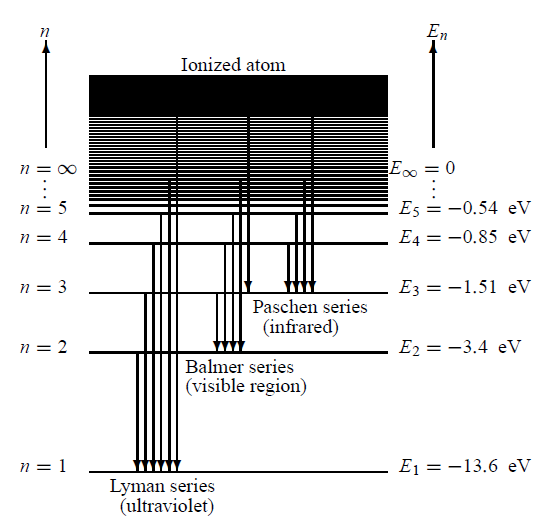
\includegraphics[width=0.45\textwidth]{Imagenes/Rydberg/transicionatomica.png}
    \caption{Saltos de energia dentro de un atomo}
    \label{fig:atomicjumps}
\end{figure}

se ha de tener en cuenta que la relación de Rydberg aplicada en este paper es solo correcta cuando tenemos átomos con solo 1 electrón libre, pues no tiene interacción potencial entre otros; para el agua que es una molécula y se compone de átomos de hidrógeno y un átomo de oxígeno, de acuerdo a la hipótesis se habría de observar una combinación del espectro del hidrógeno y oxígeno más un porcentaje de desviación pequeño debido a interacciones internas.

\section{Montaje Experimental}

\subsection{Herramientas}
\begin{itemize} 
\item Telescopio
\item Lámpara con distintas ampolletas con elementos a analizar
\item Lona para cubrir luz externa
\item Colimador
\item Lupa
\item Red de difracción
\item Escala con Vernier
\item Regla de Metro
\end{itemize}

El montaje experimental se separó en dos objetivos, el primer montaje se concentra en medir los ángulos para las líneas espectrales del hidrógeno; el segundo montaje se concentra en utilizar un método más mecánico para observar y medir las líneas espectrales del vapor de agua y mercurio.

\subsection{Experimento 1: Constante de Rydberg del Hidrógeno}
\begin{figure}[H]
    \centering
    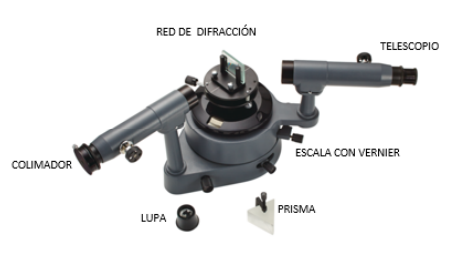
\includegraphics[width=0.45\textwidth]{Imagenes/Rydberg/experimentolabrydberg.png}
    \caption{Montaje experimento constante de Rydberg}
    \label{fig:montajeHidrogeno}
\end{figure}

Teniendo en cuenta que se desea la menor cantidad de luz se debe de cubrir con una lona todo, el telescopio utilizado posee una escala de Vernier para medir los ángulos, de manera que el experimentador observó las líneas de emisión de la lámpara de hidrógeno cuya luz atravesó el colimador; se ha de notar que entre el telescopio y la lámpara se deja una grilla de difracción tal como muestra el diagrama.

Estas líneas fueron anotadas y entonces en el análisis promediado, con el uso de scripts de Python en \cite{github} es posible despejar la longitud de onda para color. Entonces, mediante la simulación adjunta en los scripts, se consiguieron valores de la constante de Rydberg para cada dato. El lector puede visitar la sección de análisis del Mercurio para ver sobre el método gráfico, esencial cuando no se conoce el segundo nivel de energía del átomo, donde ocurre el salto entre el nivel de energía correspondiente a los electrones de valencia.

\subsection{Experimento 2: Vapor de Agua y Mercurio}
\begin{figure}[H]
    \centering
    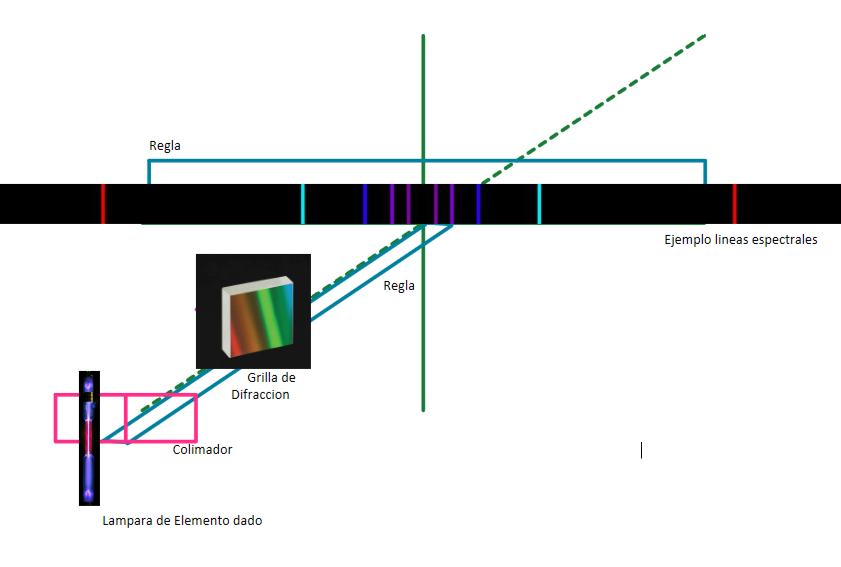
\includegraphics[width=0.45\textwidth]{Imagenes/Rydberg/experimentorydberg_agua_mercurio.png}
    \caption{Montaje que proyecta las lineas espectrales}
    \label{fig:rydbergmercury}
\end{figure}
Sígase el esquema presentado, este experimento se realizó sin el telescopio y escala de Vernier para los ángulos, como alternativa menos costosa, conservando un excelente grado de precisión.

Mediante el montaje, al prender la lámpara, la luz atravesó la grilla y el sistema óptico para alcanzar la barra donde se proyectaron las luces, entonces con la ayuda de un láser y otro experimentador, se consiguió anotar la posición de cada línea espectral, guardando el color y posición.

Las líneas espectrales del agua se compararon con las del hidrógeno, mientras que a las líneas del mercurio se les hizo una regresión lineal luego de linealizar el modelo, todos los errores fueron calculados basándonos en la mitad de la medida mínima de cada instrumento de medición y utilizando el script de Python para propagación de errores: \cite{github:errores}

\section{Análisis}
Tenemos aquí los datos del hidrógeno trabajados de manera que se observan las distintas longitudes de onda, los cuales fueron observados mediante el montaje del telescopio, promediando los ángulos y utilizando la relación de difracción \ref{eq:difraccion} se calcularon las longitudes de onda

\begin{table}[H]
\begin{tabular}{|l|l|l|l|l|} \hline
$\theta_{der}$&$\theta_{izq}$&Orden&$\lambda[nm]$&Color\\ \hline
14.4 & 14.9 & 1 & 421.52 & violeta    \\ \hline
15.4 & 15.5 & 1 & 444.0  & violeta    \\ \hline
17.4 & 17.5 & 1 & 499.79 & celeste \\ \hline
53.4 & 53.6 & 1 & 669.88 & rojo \\ \hline
23.4 & 24.0 & 2 & 439.13 & violeta    \\ \hline
36.2 & 36.5 & 2 & 493.93 & celeste \\ \hline
53.4 & 53.6 & 2 & 669.88 & rojo \\ \hline
\end{tabular}
\caption{Ángulos de las líneas espectrales del Hidrógeno}
\end{table}

Y los datos que fueron obtenidos mediante el proceso de proyectar las líneas sobre una superficie, son los siguientes:
para el vapor de agua:
\begin{table}[H]
\centering
\begin{tabular}{|llr|}
\hline
color   & Diqz[cm]                   & \multicolumn{1}
{l|}{Dder[cm] }  \\
\hline
celeste   & 79.5                   & 20                        \\
violeta   & 75.5                   & 23.8                      \\
verde     & 82.5                   & 17                        \\
roja ten  & 87.5                   & 12.5                      \\
roja main & \multicolumn{1}{r}{91} & 8   \\                   \hline  
\end{tabular}
\caption{Vapor de Agua Distancias de las líneas espectrales}
\end{table}

Para el Mercurio:
\begin{table}[H]
\centering
\begin{tabular}{|llr|}
\hline
color   & Diqz[cm]                   & \multicolumn{1}
{l|}{Dder[cm] }  \\
\hline
violeta & 72.5                   & 28.5                      \\
verde   & \multicolumn{1}{r}{78} & 22.5                      \\
naranja & \multicolumn{1}{r}{80} & 20.5                      \\
roja    & 87.5                   & 13.5   \\                   \hline
\end{tabular}
\caption{Mercurio Distancias de las líneas espectrales}
\end{table}

\subsection{Trabajando / Limpiando los datos}
para el análisis de estos se realiza el corrimiento con el offset medido de $50[cm]$, de manera que se midan desde el centro, se promedian estas dos medidas que serán casi idénticas y se consigue la distancia desde el centro llamada $D$, con esta y la distancia del difractor a la superficie $L = 95[cm]$, se calcula el seno del ángulo en que se encuentra la línea proyectada, así las siguientes tablas:

\begin{table}[H]
\centering
\begin{tabular}{|lrr|} 
\hline
color     & \multicolumn{1}{l}{D} & \multicolumn{1}{l|}{lambda [m]}  \\ 
\hline
violeta   & 25.85                 & 4.37E-07                        \\
celeste   & 29.75                 & 4.91E-07                        \\
verde     & 32.75                 & 5.49E-07                        \\
roja tenue & 37.5                  & 6.12E-07                        \\
roja fuerte & 41.5                  & 6.67E-07                        \\
\hline
\end{tabular}
\caption{Vapor de agua, datos analizados}
\end{table}

\begin{table}[H]
\centering
\begin{tabular}{|lrr|}
\hline
color   & \multicolumn{1}{l}{D [cm]} & \multicolumn{1}{l|}{lambda [m]}  \\
\hline
violeta & 22                         & 3.76E-07                                       \\
verde   & 27.75                      & 4.67E-07                                       \\
naranja & 29.75                      & 4.98E-07                                       \\
roja    & 37                         & 6.05E-07    \\    \hline              
\end{tabular}
\caption{Datos de mercurio analizados}
\label{table:mercurio}
\end{table}

entonces teniendo en cuenta \ref{eq:rydberg} conociendo qué saltos corresponden a cuáles y relacionándolos a la longitud de onda, es posible obtener la constante de Rydberg para dicho elemento.

\subsection{Rydberg para Hidrogeno}
Asumiendo serie de Balmer y la inversa de la longitud de onda, podemos relacionar cada medida a una constante de Rydberg
\begin{figure}[H]
    \centering
    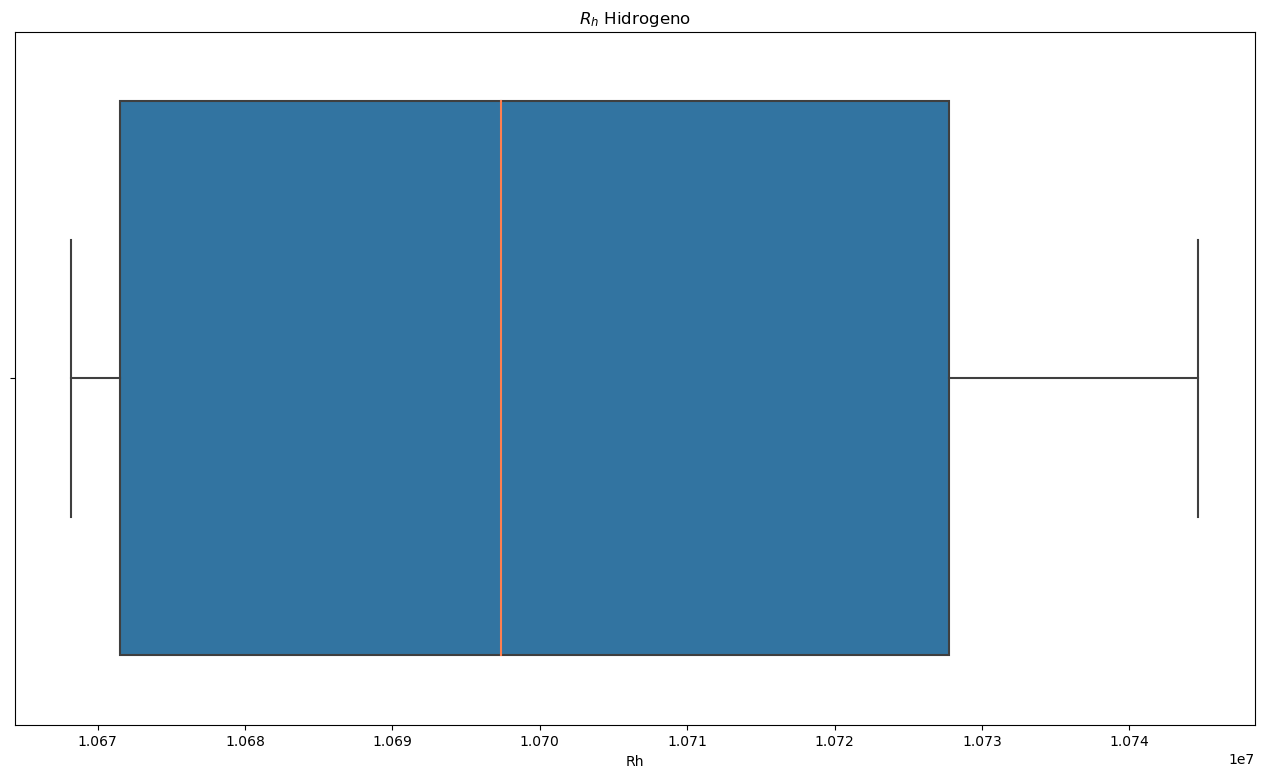
\includegraphics[width=0.5\textwidth]{Plots/Rydberg/Rh.png}
    \caption{Distribución de la constante de Rydberg para el hidrogeno}
    \label{plot:Rh}
\end{figure}
si se toma el promedio de las medidas de Rydberg, obtendríamos un promedio: $R_H = 10 701 915.8$, compara


La propagación de errores, dado que $L, D$ tengan un error de medio centímetro $0.5/100$, entonces la longitud de onda tendrá un error de $\Delta \lambda = 20 [nm]$, con esta información, la constante de Rydberg calculada usando esa incertidumbre posee un error sobre el $95\%$ de confianza de: $\Delta R_H = 2 \times 10^5 [m^{-1}]$

cada medición comparada a la constante de Rydberg teórica \ref{eq:rydberg}, $R^T_H = 10 973 731.6$
\begin{figure}[H]
    \centering
    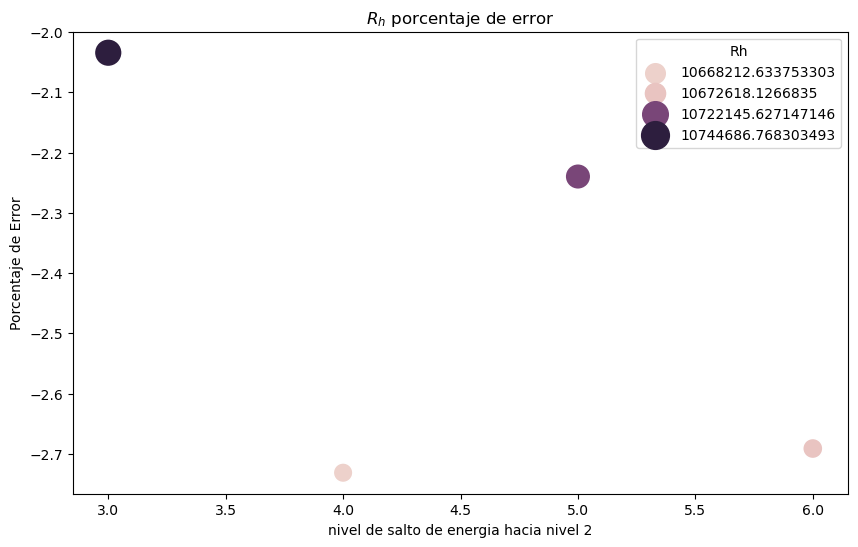
\includegraphics[width=0.5\textwidth]{Plots/Rydberg/porcntErrorPorSalto.png}
    \caption{Diferencia de Rydberg calculado comparado a la constante de Rydberg teorica}
    \label{plot:RhError}
\end{figure},

\subsection{Análisis de la Molécula de Agua}

En el caso del agua se compone de átomos de hidrógeno y de oxígeno, por tanto, se hizo calzar las líneas espectrales del hidrógeno con las observadas en el agua utilizando un algoritmo de Python que itera en diferencias porcentuales permitidas y entrega un dataframe ordenado, puede encontrar el algoritmo en el github de los escritores: \cite{github}

\begin{table}[H]
\centering
\begin{tabular}{|l|r|r|r|}
\hline
color $H_2O$     & \multicolumn{1}{l}{$H_2O$ [nm]} & \multicolumn{1}{|l|}{H [nm]} & \multicolumn{1}{l|}{$\epsilon$}  \\
\hline
violeta    & 437.598                            & 443.9956                                  & 0.015                                       \\
celeste    & 498.078                            & 499.789                                   & 0.005                                       \\
verde    & 543.19                             & 499.789                                   & 0.09                                        \\
rojo tenue & 611.944                            & 669.913                                   & 0.09                                        \\
roj fuerte & 667.188                            & 669.913                                   & 0.005  \\ \hline                                    
\end{tabular}
\caption{Fitting Longitud de Ondas Hidrogeno Vapor de Agua}
\end{table}

tomando los errores más pequeños, en este caso $0.005 = 0.5 \% $, es menor a un $1\%$, podemos especificar cuales son producto del hidrógeno contenido en el agua y cuales son producto del átomo de oxígeno, la siguiente tabla compara e incluye la información de los colores:


\begin{table}[H]
\centering
\begin{tabular}{|lr|ll|}
\hline
color $H_2O$ & \multicolumn{1}{l|}{$H_2O$ [nm]} & H [nm]  & color $H$     \\
\hline
violeta   & 437.59                      & \multicolumn{1}{r}{443.99} & violeta2   \\
celeste   & 498.07                      & \multicolumn{1}{r}{499.78}  & celeste     \\
verde     & 543.1                       &                              &             \\
roja 2  & 611.94                      &                              &             \\
roja 1 & 667.18                      & \multicolumn{1}{r}{669.91}  & rojo  \\
\hline
\end{tabular}
\caption{Tabla de Color Hidrógeno y Vapor de Agua}
\label{table:watercolor}
\end{table}

\subsection{Análisis del Átomo de Mercurio}
Por otro lado, átomos tan pesados como el mercurio contiene varios átomos que agregan interacciones complicando el problema, para este caso se opta por el método gráfico, para ello reescribimos la ecuación de Rydberg antes presentada (\ref{eq:rydberginit}):
$$
y = m x + b
$$
donde utilizamos los datos medidos dentro del $y$
$$
y = \frac{1}{\lambda}
$$
luego tomando un rango de valores de n para utilizarlos como x, $x = 1/n^2$, $m= R_{Hg}$ y el intercepto $b= - R_{Hg} / m^2$
$$
m x + b = R_{Hg} \frac{1}{n^2} - R_{Hg} / m^2
$$

mediante la regresión lineal mediante mínimos cuadrados se obtiene el intercepto, la pendiente, el coeficiente de relación de pearson, que elevado al cuadrado indica cual es el porcentaje de datos que se explican mediante la regresión ($r^2 = 95.3 \% $), utilizando test de hipótesis para el intercepto, se despeja el intervalo de confianza del $95\%$ para la pendiente:
$$m = R_{Hg} = 0.011073 \pm 0.005526 $$

\section{Conclusión}
Se consiguio asi, analizar estos 3 casos de emisión utilizando leyes basicas de cuantica, reglas de cuantización en especifico. Se consiguió calcular la constante de Rydberg para el hidrogeno $R_H = 10701915.785 \pm 2 \times 10^5 [m^{-1}]$, sin embargo aun contando el error la constante teorica no se encuentra dentro de ese rango. El error porcentual comparado a la constante teorica es un error de $0.6 \%$

\subsection{Vapor de Agua e Hidrógeno}
Observando la tabla *\ref{table:watercolor}
teniendo en cuenta los errores, comparado a un grado de confianza del $95\%$ para el test de hipotesis: los datos se explican, las lineas espectrales de una molécula se comparan a las de sus átomos que la componen. Usando una diferencia relativa entre las longitudes de onda menor al $1.5\%$ como ideal; notar que diferencias como las del $9\%$ procedían a tomar datos ya asignados a errores mucho menores, por tanto se recomienda utilizar el algoritmo \cite{github} con un $epsilonLimit \leq 0.09 - 0.015$ osea con un $epsilonLimit \leq 7.5 \%$.


\subsection{Mercurio}
Para el mercurio, debido a interacciones internas y grandes diferencias a como se comporta la emisión del hidrógeno, no se logró un 'fit' con un error dentro de los estándares recomendados; sin embargo el método gráfico consiguió rápidamente la constante de Rydberg para este elemento teniendo en cuenta hasta 6 niveles de energía:
 $$ R_{Hg} = 0.011073 \pm 0.005526 $$ con un $95\%$ de confianza estadística.

Si el lector gusta complementar información, léase \cite{thornton}

\medskip

\printbibliography

\end{document}

 